

\numberwithin{equation}{section}

\section{Penalty Matrix in (\ref{tractormse})}\label{PenaltyTermDetails}

The $i$-th $\Omega^{(i)}$ is a $2n \times 2n$ bandwidth four symmetric matrix and its non-zero elements on the upper triangular are in the form of
\begin{align}
\Omega_{2i-1,2i-1}^{(i)} & =\int_{t_{i}}^{t_{i+1}} \frac{d^2 h_{00}^{(i)}(t)}{dt^2}  \frac{d^2 h_{00}^{(i)}(t)}{dt^2} dt=\frac{12}{\Delta_i^3}\\
\Omega_{2i-1,2i}^{(i)} &=\int_{t_{i}}^{t_{i+1}} \frac{d^2 h_{00}^{(i)}(t)}{dt^2}  \frac{d^2 h_{10}^{(i)}(t)}{dt^2} dt=\frac{6}{\Delta_i^2}\\
\Omega_{2i-1,2i+1}^{(i)} &=\int_{t_{i}}^{t_{i+1}} \frac{d^2 h_{00}^{(i)}(t)}{dt^2}  \frac{d^2 h_{01}^{(i+1)}(t)}{dt^2} dt=\frac{-12}{\Delta_i^3}\\
\Omega_{2i-1,2i+2}^{(i)} &=\int_{t_{i}}^{t_{i+1}} \frac{d^2 h_{00}^{(i)}(t)}{dt^2}  \frac{d^2 h_{11}^{(i+1)}(t)}{dt^2} dt=\frac{6}{\Delta_i^2}\\
\Omega_{2i,2i}^{(i)} &=\int_{t_{i}}^{t_{i+1}} \frac{d^2 h_{10}^{(i)}(t)}{dt^2}  \frac{d^2 h_{10}^{(i)}(t)}{dt^2} dt=\frac{4}{\Delta_i} \\
\Omega_{2i,2i+1}^{(i)} &=\int_{t_{i}}^{t_{i+1}} \frac{d^2 h_{10}^{(i)}(t)}{dt^2}  \frac{d^2 h_{01}^{(i+1)}(t)}{dt^2} dt=\frac{-6}{\Delta_i^2}\\
\Omega_{2i,2i+2}^{(i)} &=\int_{t_{i}}^{t_{i+1}} \frac{d^2 h_{10}^{(i)}(t)}{dt^2}  \frac{d^2 h_{11}^{(i+1)}(t)}{dt^2} dt=\frac{2}{\Delta_i}\\
\Omega_{2i+1,2i+1}^{(i)} &=\int_{t_{i}}^{t_{i+1}} \frac{d^2 h_{01}^{(i+1)}(t)}{dt^2}  \frac{d^2 h_{01}^{(i+1)}(t)}{dt^2} dt=\frac{12}{\Delta_i^3}\\
\Omega_{2i+1,2i+2}^{(i)} &=\int_{t_{i}}^{t_{i+1}} \frac{d^2 h_{01}^{(i+1)}(t)}{dt^2}  \frac{d^2 h_{11}^{(i+1)}(t)}{dt^2} dt=\frac{-6}{\Delta_i^2}\\
\Omega_{2i+2,2i+2}^{(i)} &=\int_{t_{i}}^{t_{i+1}} \frac{d^2 h_{11}^{(i+1)}(t)}{dt^2}  \frac{d^2 h_{11}^{(i+1)}(t)}{dt^2} dt=\frac{4}{\Delta_i}
\end{align}
where $\Delta_i=T_{i+1}-T_i$ and $i=1,2,\ldots,n-1$. Then 
\begin{equation*}
\mathbf{\Omega}=\sum_{i=1}^{n-1}\lambda_i\Omega^{(i)}
\end{equation*}



\section{Proof of Theorem \ref{basisindependent}}\label{AppendixBasisproof}

\begin{proof}
It is obvious that these basis functions are continuous on subinterval $[t_k,t_{k+1}]$. We will prove that these basis functions are independent at first. 

Given $2n$ basis functions and $n$ knots, we choose $t_1, \frac{t_1+t_2}{2}, t_2, \frac{t_2+t_3}{2}, \cdots, t_{n-1}$, $\frac{t_{n-1}+t_n}{3}$, $\frac{2(t_{n-1}+t_n)}{3}, t_n$ as new $2n$ knots, and denoted by $c_1,c_2,\cdots,c_{2n}$. Then the determinant is
\begin{align}\label{matrixD}
\begin{split}
D(c_1,c_2,\cdots,c_{2n})=&
\begin{vmatrix}
N_1(c_1) & N_1(c_2) & \cdots& N_1(c_{2n})\\
N_2(c_1) & N_2(c_2)& \cdots & N_2(c_{2n})\\
 \vdots  &  \vdots  & \ddots  & \vdots  \\  
N_{2n}(c_1) & N_{2n}(c_2) & \cdots & N_{2n}(c_{2n})\\
\end{vmatrix}
\\=&
\begin{vmatrix}
1 & a_{12} & 0 & 0 & \cdots& 0 & 0 \\
0 & a_{22} & 0 & 0 & \cdots& 0 & 0\\
0 & a_{32} & 1 & a_{34} & \cdots& 0 & 0\\
 \vdots  &  \vdots  &  \vdots &  \vdots & \ddots  & \vdots   &  \vdots\\  
0 & 0 & 0 & 0 & \cdots& a_{2n-1,2n-1} & 1\\
0 & 0 & 0 & 0 & \cdots& a_{2n,2n-1} & 0 \\
\end{vmatrix},
\end{split}
\end{align}
where $D(c_1,c_2,\cdots,c_{2n})=\begin{cases}
N_1(t_1)=1 \\
N_1(\frac{t_1+t_2}{2})=a_{12} \\
N_2(t_1)=0 \\
N_2(\frac{t_1+t_2}{2})=a_{22} \\
N_{2k+1}(\frac{t_k+t_{k+1}}{2})=a_{2k+1,2k} & k=1,2,\cdots,2n \\ 
N_{2k+1}(t_{k+1})=1 & k=1,2,\cdots,2n \\ 
N_{2k+1}(\frac{t_{k+1}+t_{k+2}}{2})=a_{2k+1,2k+2} & k=1,2,\cdots,2n \\ 
N_{2k+2}(\frac{t_k+t_{k+1}}{2})=a_{2k+2,2k} & k=1,2,\cdots,2n \\ 
N_{2k+2}(\frac{t_{k+1}+t_{k+2}}{2})=a_{2k+2,2k+2}  & k=1,2,\cdots,2n\\ 
N_{2n-1}(t_{2n-1})=0 \\
N_{2n-1}(\frac{t_{2n-1}+t_{2n}}{3})=a_{2n-1,2n-2} \\
N_{2n-1}(\frac{2(t_{2n-1}+t_{2n})}{3})=a_{2n-1,2n-1} \\
N_{2n-1}(t_{2n})=1 \\
N_{2n}(\frac{t_{2n-1}+t_{2n}}{3})=a_{2n,2n-2} \\
N_{2n}(\frac{2(t_{2n-1}+t_{2n})}{3})=a_{2n,2n-1} \\
N_{2n}(t_{2n})=0 \\
0 &  \mbox{otherwise}
\end{cases}$,\\
and $a_{ij}\neq 0.$ After decomposing determinant $D$ in equation (\ref{matrixD}),  gives
\begin{align*}
\det D= & 
\begin{vmatrix}
 a_{22} & 0 & 0 & \cdots& 0 & 0\\
 a_{32} & 1 & a_{34} & \cdots& 0 & 0\\
  \vdots  &  \vdots &  \vdots & \ddots  & \vdots   &  \vdots\\  
0 & 0 & 0 & \cdots& a_{2n-1,2n-1} & 1\\
0 & 0 & 0 & \cdots& a_{2n,2n-1} & 0 \\
\end{vmatrix}
=a_{22}
\begin{vmatrix}
 1 & a_{34} & \cdots& 0 & 0\\
  \vdots &  \vdots & \ddots  & \vdots   &  \vdots\\  
 0 & 0 & \cdots& a_{2n-1,2n-1} & 1\\
 0 & 0 & \cdots& a_{2n,2n-1} & 0 \\
\end{vmatrix}\\
=& \cdots =a_{22}a_{44}\cdots a_{2n-4,2n-4} 
\begin{vmatrix}
a_{2n-2,2n-2} & a_{2n-2,2n-1}  & 0\\
a_{2n-1,2n-2} & a_{2n-1,2n-1} & 1\\
 a_{2n,2n-2} &  a_{2n,2n-1} & 0 \\
\end{vmatrix}\\
=& a_{22}a_{44}\cdots a_{2n-4,2n-4} (a_{2n-2,2n-1}a_{2n,2n-2}-a_{2n,2n-1}a_{2n-2,2n-2}) \neq 0.
\end{align*}
With the conclusion in Lemma 1, $N_1(t),\ldots,N_{2n}(t)$  are linearly independent on interval $[t_1, t_n]$.
Secondly, we prove that basis functions represent any cubic function on each interval $[t_k, t_{k+1}]$. Due to the definition of cubic spline, on interval $[t_k, t_{k+1}]$, a cubic spline $g(t)$ can be written in the form of
\begin{eqnarray}
g(t)=d_k (t-t_k)^3+c_k(t-t_k)^2+b_k(t-t_k)+a_k, \mbox{for $t_k \leq t \leq t_{k+1}$}
\end{eqnarray}
For any $f(t)$ on $[t_1, t_n]$, it can be represented as $f(t)=\sum_{k=1}^{2n} \theta_k N_k(t)$. Then for $\forall t \in [t_k,t_{k+1}]$, we have
\begin{align*}
f(t)=\begin{cases}
\theta_{2k-1}N_{2k-1}(t)+\theta_{2k}N_{2k}(t)+\theta_{2k+1}N_{2k+1}(t)+\theta_{2k+2}N_{2k+3}(t), & t_k \leq t \leq t_{k+1}  \\
0, & \mbox{otherwise}\\
\end{cases},
\end{align*}
thus
\begin{align*}
f(t)=&\theta_{2k-1}\{ 2(\frac{t-t_{k}}{t_{k+1}-t_{k}})^3-3(\frac{t-t_{k}}{t_{k+1}-t_{k}})^2+1  \} \\+&\theta_{2k} \{  \frac{(t-t_{k})^3}{(t_{k+1}-t_{k})^2}-2\frac{(t-t_{k})^2}{t_{k+1}-t_{k}}+(t-t_{k}) \} \\
+&\theta_{2k+1} \{ -2(\frac{t-t_k}{t_{k+1}-t_k})^3+3(\frac{t-t_k}{t_{k+1}-t_k})^2  \}  +\theta_{2k+2} \{  \frac{(t-t_k)^3}{(t_{k+1}-t_k)^2}-\frac{(t-t_k)^2}{t_{k+1}-t_k} \}.
\end{align*}
After rearranging, we have
\begin{align*}
f(t)=& \{ \frac{2\theta_{2k-1}}{(t_{k+1}-t_{k})^3} +\frac{\theta_{2k}}{(t_{k+1}-t_{k})^2} -\frac{2\theta_{2k+1}}{(t_{k+1}-t_{k})^3} +\frac{\theta_{2k+2}}{(t_{k+1}-t_{k})^2} \} (t-t_k)^3 \\
+&  \{ -\frac{3\theta_{2k-1}}{(t_{k+1}-t_{k})^2} -\frac{2\theta_{2k}}{(t_{k+1}-t_{k})} +\frac{3\theta_{2k+1}}{(t_{k+1}-t_{k})^2} - \frac{\theta_{2k+2}}{(t_{k+1}-t_{k})} \} (t-t_k)^2 \\
+&  \theta_{2k} (t-t_k) +\theta_{2k-1},
\end{align*}
where coefficients are
\begin{align*}
\begin{cases}
\theta_{2k-1}=a_k\\
\theta_{2k}=b_k\\
-\frac{3\theta_{2k-1}}{(t_{k+1}-t_{k})^2} -\frac{2\theta_{2k}}{(t_{k+1}-t_{k})} +\frac{3\theta_{2k+1}}{(t_{k+1}-t_{k})^2} - \frac{\theta_{2k+2}}{(t_{k+1}-t_{k})}=c_k\\
\frac{2\theta_{2k-1}}{(t_{k+1}-t_{k})^3} +\frac{\theta_{2k}}{(t_{k+1}-t_{k})^2} -\frac{2\theta_{2k+1}}{(t_{k+1}-t_{k})^3} +\frac{\theta_{2k+2}}{(t_{k+1}-t_{k})^2}=d_k
\end{cases}
\end{align*}
the resulting can always be solved for $\theta_{2k-1}, \theta_{2k},\theta_{2k+1},\theta_{2k+2}$ in terms of $a_k,b_k,c_k,d_k$ on interval $[t_k, t_{k+1}]$. So cubic spline on each interval can be represented by basis functions. \\

Finally, we will prove basis functions are continuous on $[t_1, t_n]$. For any knot $t_k$, where $t_1< t_k <t_n$, it is known that $f(t_k)=\theta_{2k-1}$. Moreover, 
\begin{align*}
\lim\limits_{t\rightarrow t_k+} f(t) = \lim\limits_{t\rightarrow t_k+} (\theta_{2k-1}N_{2k-1}(t)+\theta_{2k}N_{2k}(t)+\theta_{2k+1}N_{2k+1}(t)+\theta_{2k+2}N_{2k+3}(t))=\theta_{2k-1},\\
\lim\limits_{t\rightarrow t_k-} f(t) = \lim\limits_{t\rightarrow t_k-} (\theta_{2k-1}N_{2k-1}(t)+\theta_{2k}N_{2k}(t)+\theta_{2k+1}N_{2k+1}(t)+\theta_{2k+2}N_{2k+3}(t))=\theta_{2k-1}.
\end{align*}
So
\begin{align*}
\lim\limits_{t\rightarrow t_k^+} f(t) =\lim\limits_{t\rightarrow t_k^-} f(t) =f(t),
\end{align*}
$f(t)$ is continuous at knots, and then continuous on whole interval $[t_1,t_n]$.
$f(t)$ is a continuous cubic spline on interval $[t_1,t_n]$, then $f(t)$ has continuous first and second derivatives.
\end{proof}

\section{Proof of Lemma \ref{cvlemma}}
\begin{proof}
For any spline $f$, 
\begin{equation}
\begin{split}
&\frac{1}{n}\sum_{j=1}^{n}(y_j^*-f(t_j))^2+\frac{\gamma}{n} \sum_{j=1}^{n}(v_j^*-f'(t_j))+\lambda\int f''^2 \\
\geq&\frac{1}{n}\sum_{j\neq i}^{n}(y_j^*-f(t_j))^2+\frac{\gamma}{n} \sum_{j\neq i}^{n}(v_j^*-f'(t_j))+\lambda\int f''^2\\
\geq&\frac{1}{n}\sum_{j\neq i}^{n}(y_j^*-\hat{f}^{(-i)}(t_j))^2+\frac{\gamma}{n} \sum_{j\neq i}^{n}(v_j^*-\hat{f}'^{(-i)}(t_j))+\lambda\int \hat{f}^{(-i)''2}\\
=&\frac{1}{n}\sum_{j=1}^{n}(y_j^*-\hat{f}^{(-i)}(t_j))^2+\frac{\gamma}{n} \sum_{j=1}^{n}(v_j^*-\hat{f}'^{(-i)}(t_j))+\lambda\int \hat{f}^{(-i)''2}
\end{split}
\end{equation}
by the definition of $\hat{f}^{(-i)}$, $\hat{f}'^{(-i)}$ and $y_i^*=\hat{f}^{(-i)}(t_i)$, $v_i^*=\hat{f}'^{(-i)}(t_i)$. It follows that $\hat{f}^{(-i)}$ is the minimizer of the MSE function (*****), so that
\begin{align}
\mathbf{\hat{f}}^{(-i)}&=S\mathbf{y}^*+\gamma T\mathbf{v}^*\\
\mathbf{\hat{f}}'^{(-i)}&=U\mathbf{y}^*+\gamma V\mathbf{v}^*
\end{align}
\end{proof}


\section{Proof of Theorem \ref{tractorsplinecvscore}}

\begin{proof}
\begin{equation}\label{th3proofeq1}
\begin{split}
\hat{f}^{(-i)}(t_i)-y_i=& \sum_{j=1}^{n}S_{ij}y_j^*+ \gamma \sum_{j=1}^{n}T_{ij}v_j^*-y_i^*\\
=&\sum_{j\neq i}^{n}S_{ij}y_j+ \gamma \sum_{j\neq i}^{n}T_{ij}v_j+S_{ii}\hat{f}^{(-i)}(t_i)+\gamma T_{ii}\hat{f}'^{(-i)}(t_i)-y_i\\
=&\sum_{j=1}^{n}S_{ij}y_j+ \gamma \sum_{j=1}^{n}T_{ij}v_j+S_{ii}(\hat{f}^{(-i)}(t_i)-y_i)+\gamma T_{ii}(\hat{f}'^{(-i)}(t_i)-v_i)-y_i\\
=&(\hat{f}(t_i)-y_i)+S_{ii}(\hat{f}^{(-i)}(t_i)-y_i)+\gamma T_{ii}(\hat{f}'^{(-i)}(t_i)-v_i).
\end{split}
\end{equation}
Additionally, 
\begin{equation}
\begin{split}
\hat{f}'^{(-i)}(t_i)-v_i=& \sum_{j=1}^{n}U_{ij}y_j^*+ \gamma \sum_{j=1}^{n}V_{ij}v_j^*-v_i^*\\
=&\sum_{j\neq i}^{n}U_{ij}y_j+ \gamma \sum_{j\neq i}^{n}V_{ij}v_j+U_{ii}\hat{f}^{(-i)}(t_i)+\gamma V_{ii}\hat{f}'^{(-i)}(t_i)-v_i\\
=&\sum_{j=1}^{n}U_{ij}y_j+ \gamma \sum_{j=1}^{n}V_{ij}v_j+U_{ii}(\hat{f}^{(-i)}(t_i)-y_i)+\gamma V_{ii}(\hat{f}'^{(-i)}(t_i)-v_i)-v_i\\
=&(\hat{f}'(t_i)-v_i)+U_{ii}(\hat{f}^{(-i)}(t_i)-y_i)+\gamma V_{ii}(\hat{f}'^{(-i)}(t_i)-v_i).
\end{split}
\end{equation}
Then
\begin{equation}\label{th3proofeq2}
\hat{f}'^{(-i)}(t_i)-v_i = \frac{\hat{f}'(t_i)-v_i}{1-\gamma V_{ii}}+ \frac{U_{ii}(\hat{f}^{(-i)}(t_i)-y_i)}{1-\gamma V_{ii}}.
\end{equation}
After substituting equation (\ref{th3proofeq2}) into (\ref{th3proofeq1}), we get
\begin{equation}
\hat{f}^{(-i)}(t_i)-y_i=\frac{\hat{f}(t_i)-y_i+\gamma \frac{T_{ii}}{1-\gamma V_{ii}}(\hat{f}'(t_i)-v_i)}{1-S_{ii}-\gamma\frac{T_{ii}}{1-\gamma V_{ii}}U_{ii}}.
\end{equation}
Then
\begin{equation}
CV(\lambda,\gamma)=\frac{1}{n}\sum_{i=1}^{n}\frac{\hat{f}(t_i)-y_i+\gamma \frac{T_{ii}}{1-\gamma V_{ii}}(\hat{f}'(t_i)-v_i)}{1-S_{ii}-\gamma\frac{T_{ii}}{1-\gamma V_{ii}}U_{ii}}.
\end{equation}
\end{proof}


\clearpage

\section{Residuals Analysis}
\begin{figure}[!ht]
    \centering
    \begin{subfigure}{0.45\textwidth}
    \centering
    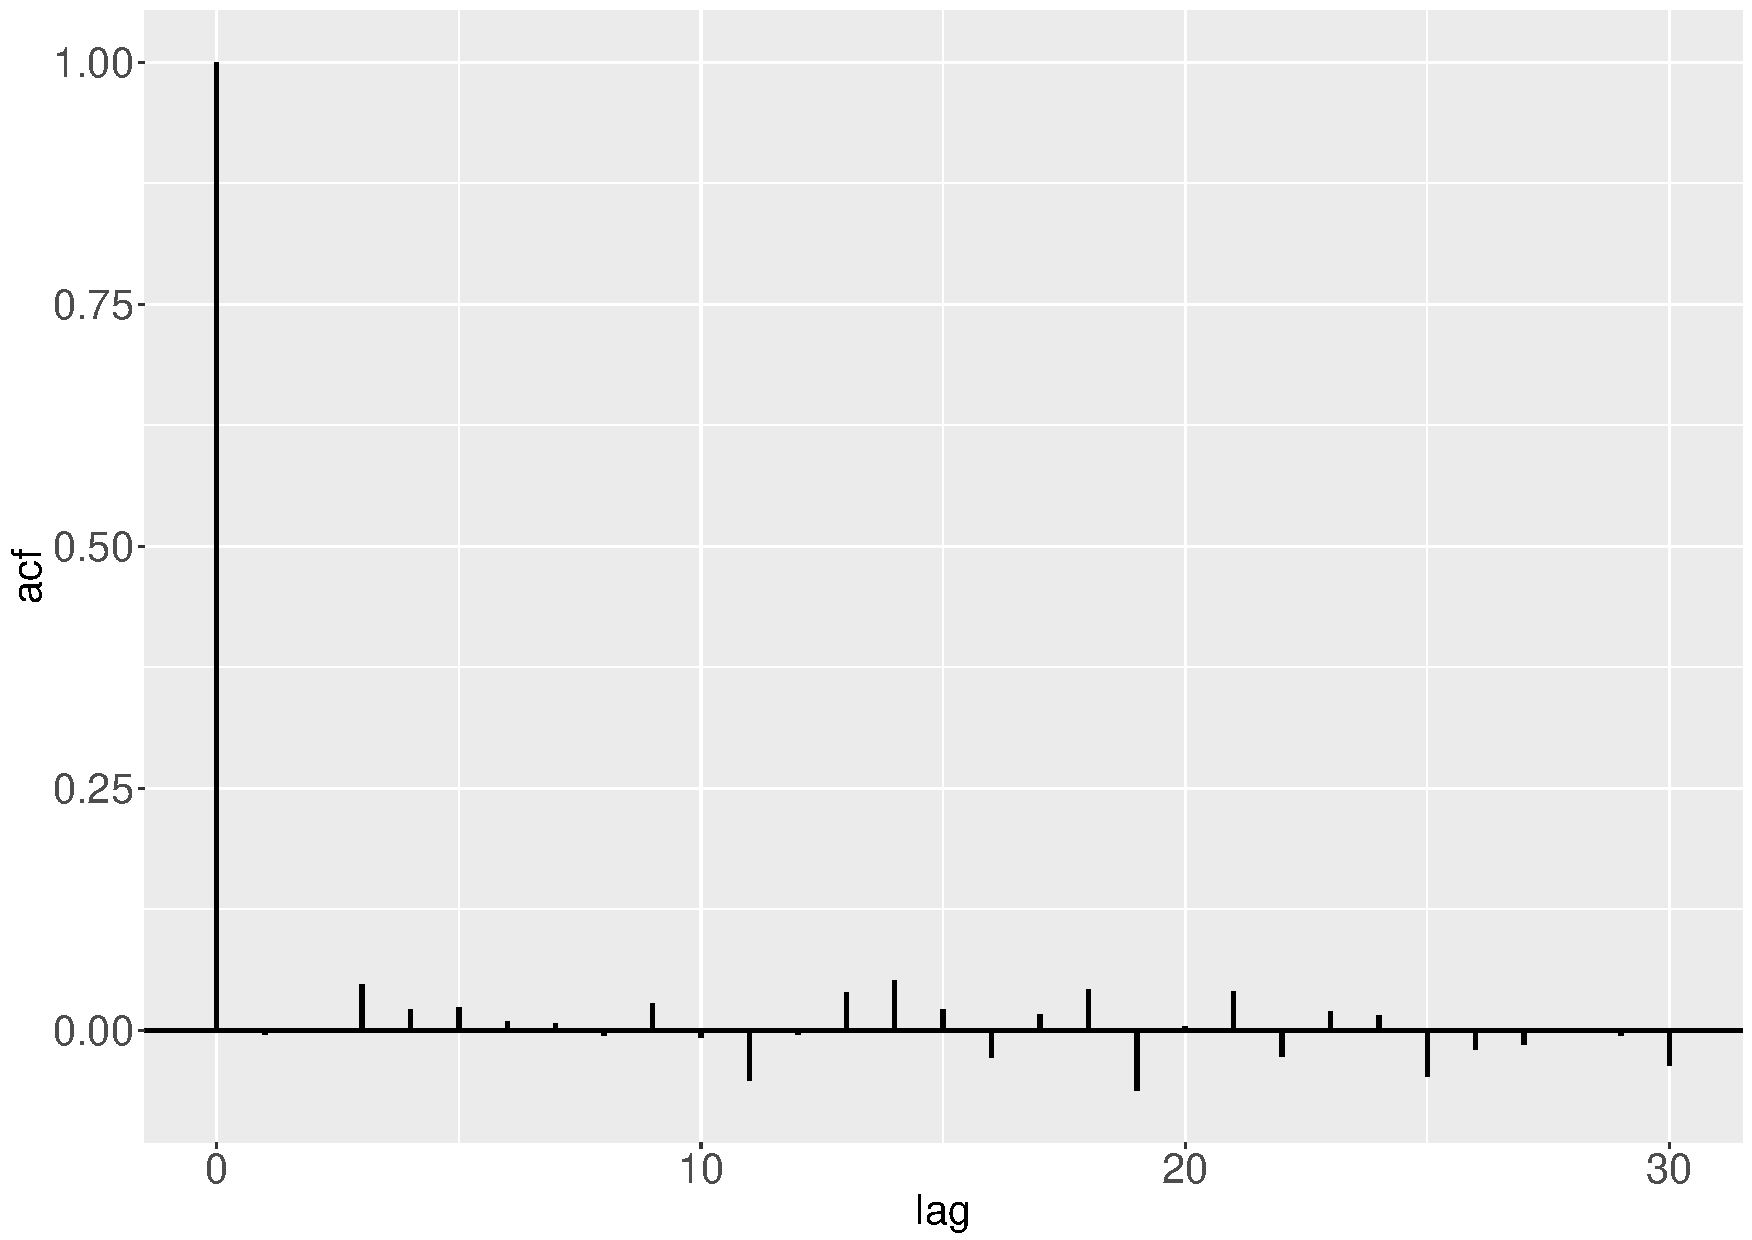
\includegraphics[width=\textwidth]{Chapters/02TractorSplineTheory/plot/ggplot/ggacfBlocks7.pdf}
    \caption{ACF of residuals from \textit{Blocks} with SNR at 7 }
    \end{subfigure}%
    \begin{subfigure}{0.45\textwidth}
    \centering
    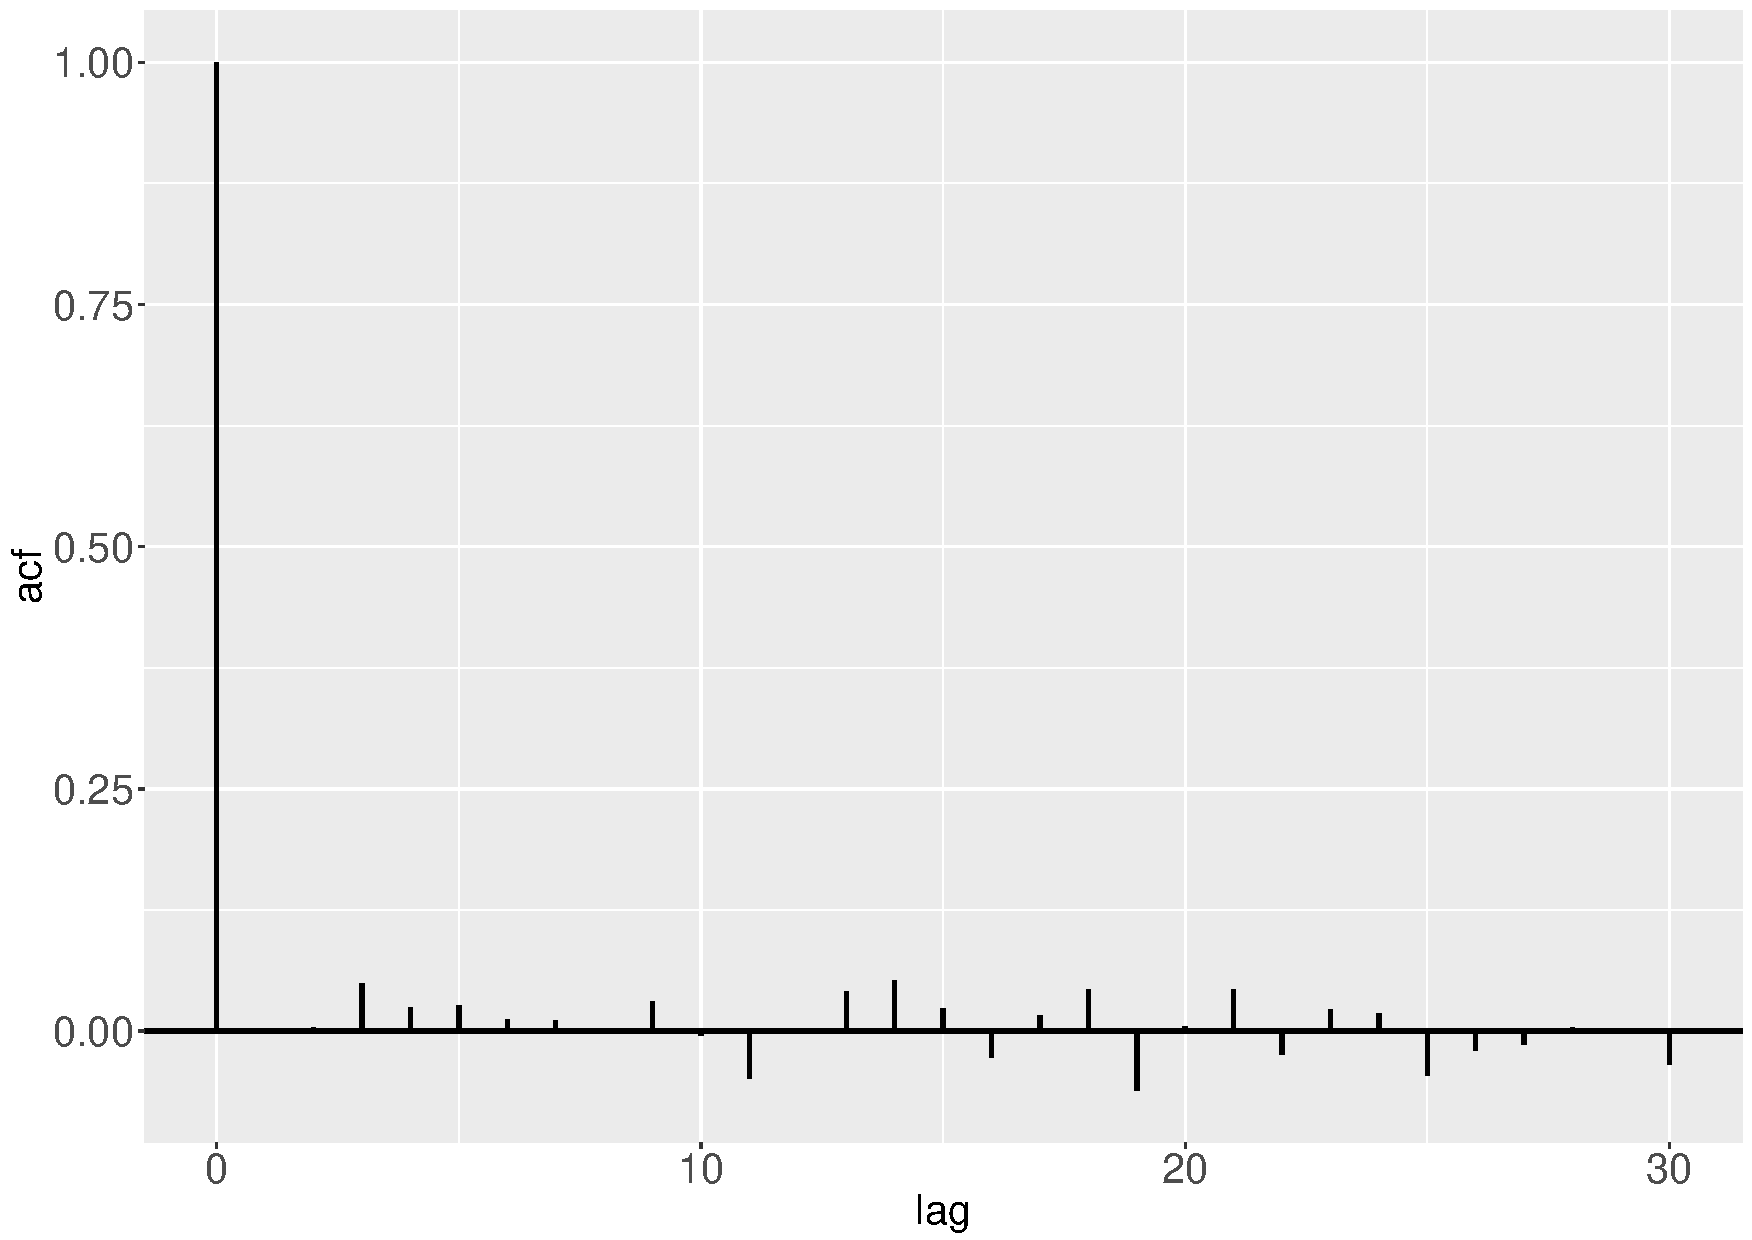
\includegraphics[width=\textwidth]{Chapters/02TractorSplineTheory/plot/ggplot/ggacfBumps7.pdf}
    \caption{ACF of residuals from \textit{Bumps} with SNR at 7 }
    \end{subfigure}
    \begin{subfigure}{0.45\textwidth}
    \centering
    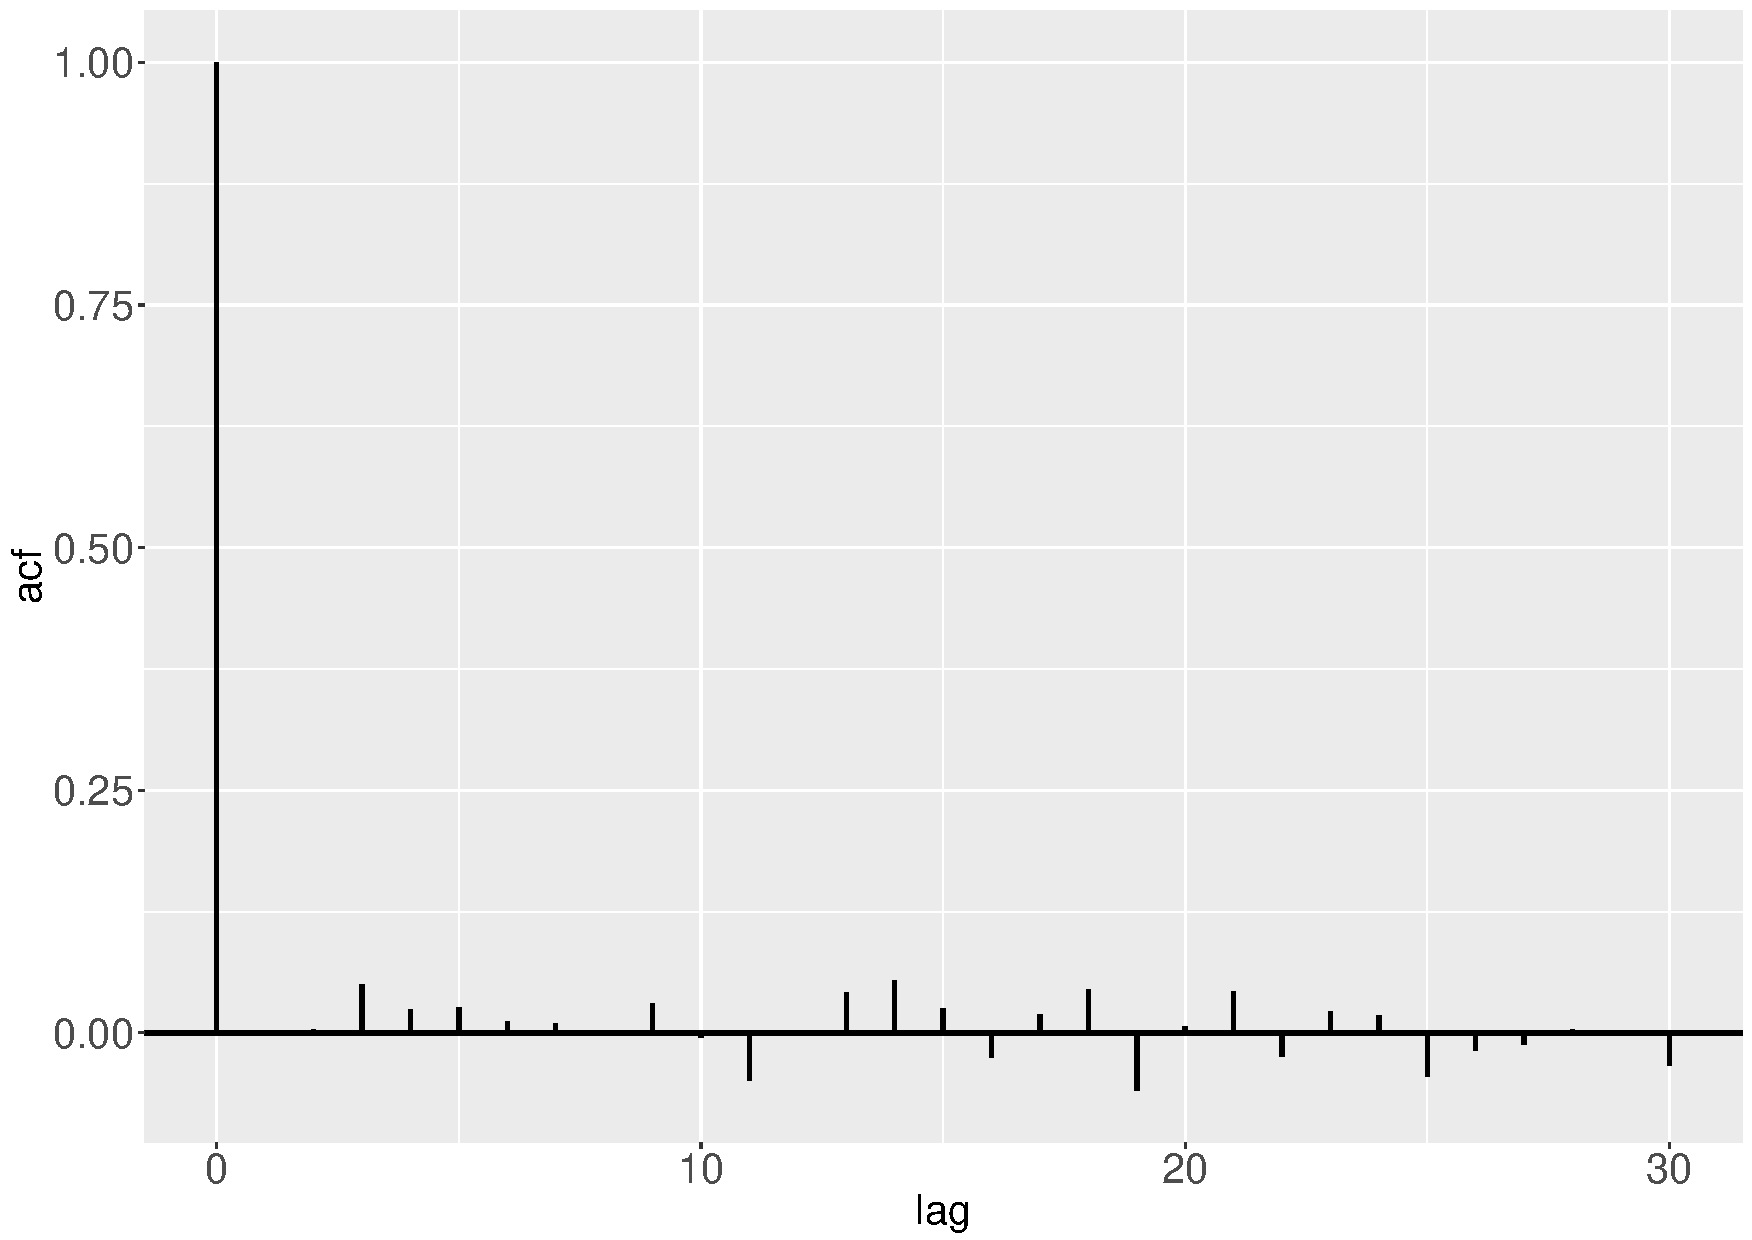
\includegraphics[width=\textwidth]{Chapters/02TractorSplineTheory/plot/ggplot/ggacfHeavi7.pdf}
    \caption{ACF of residuals from \textit{HeaviSine} with SNR at 7 }
    \end{subfigure}
    \begin{subfigure}{0.45\textwidth}
    \centering
    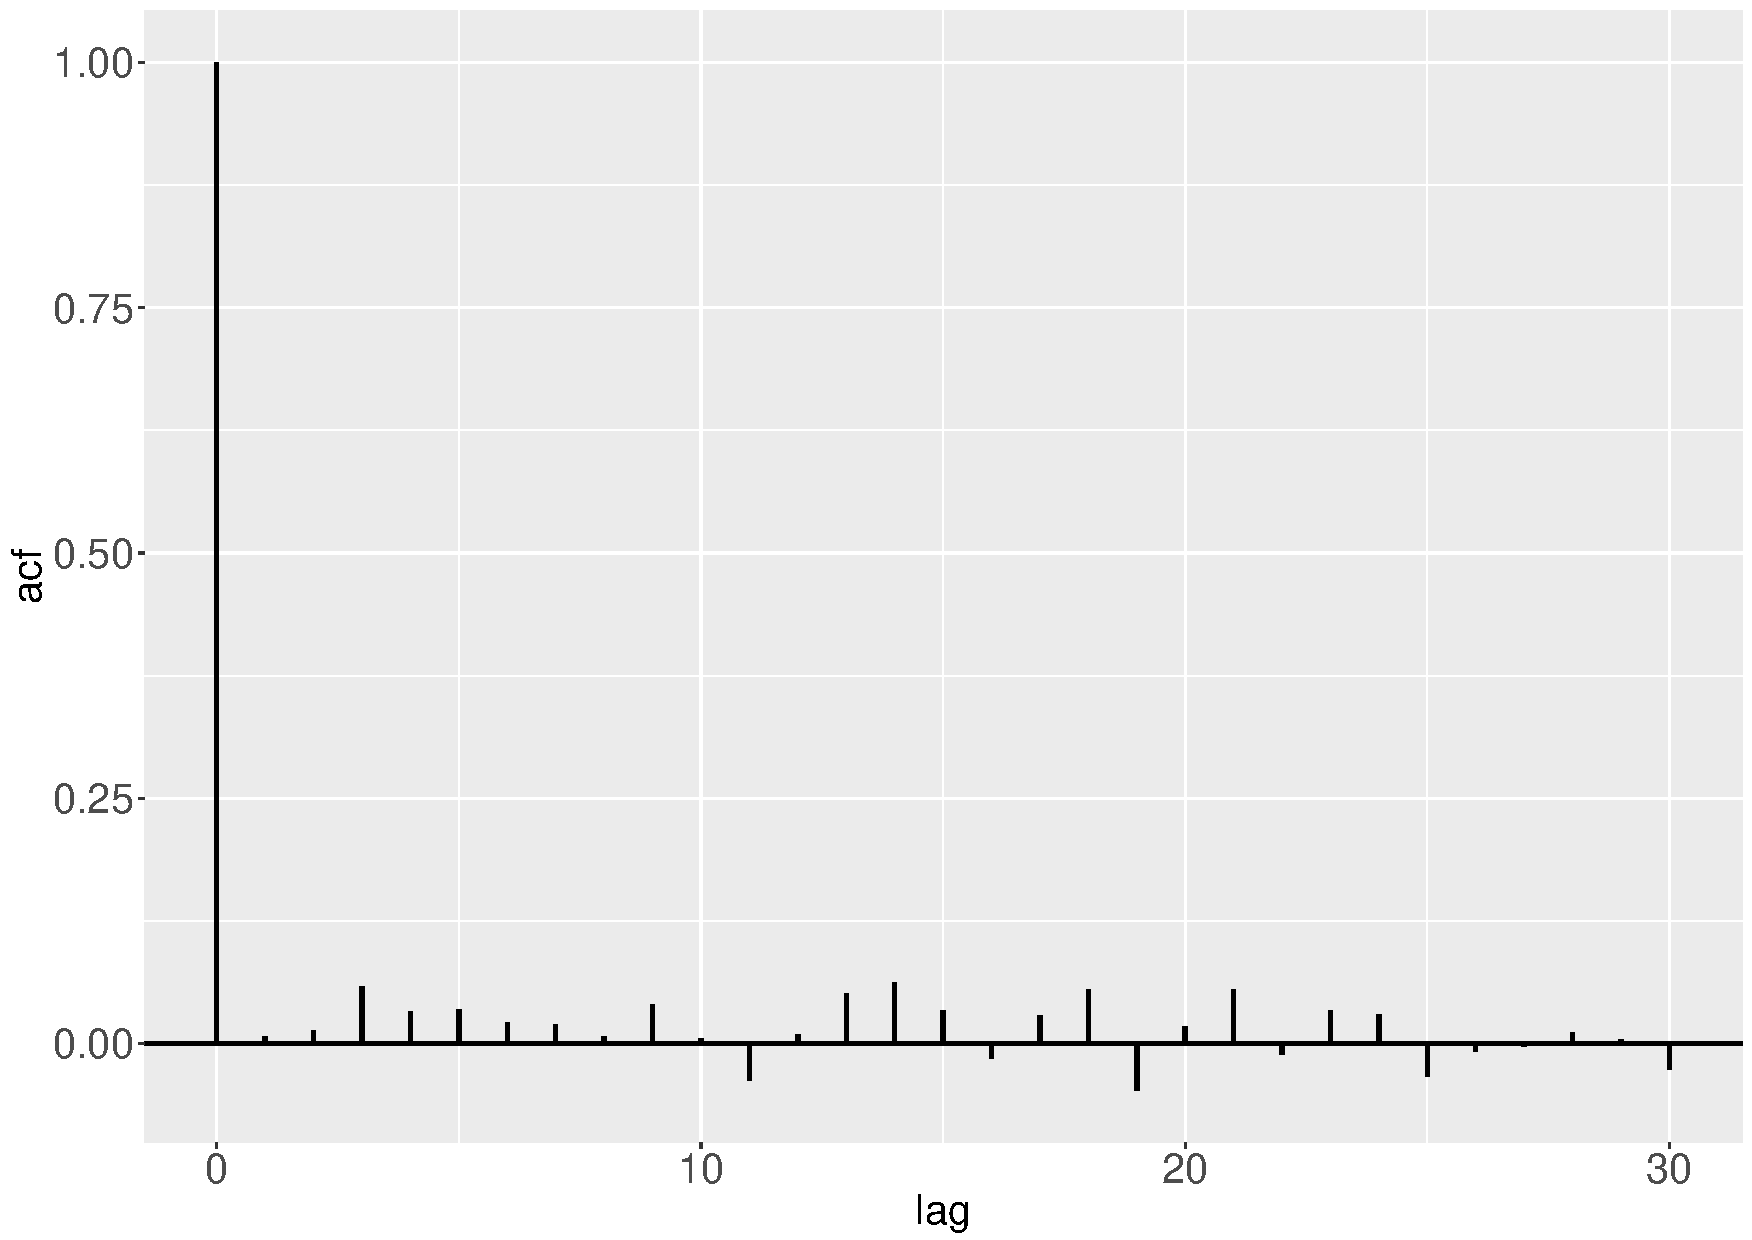
\includegraphics[width=\textwidth]{Chapters/02TractorSplineTheory/plot/ggplot/ggacfDoppler7.pdf}
    \caption{ACF of residuals from \textit{Doppler} with SNR at 7 }
    \end{subfigure}
\caption{ACF of residuals at SNR level of 7.}\label{tractorsplineSNR7acf}
 \end{figure}
\begin{figure}[!ht]
    \centering
    \begin{subfigure}{0.45\textwidth}
    \centering
    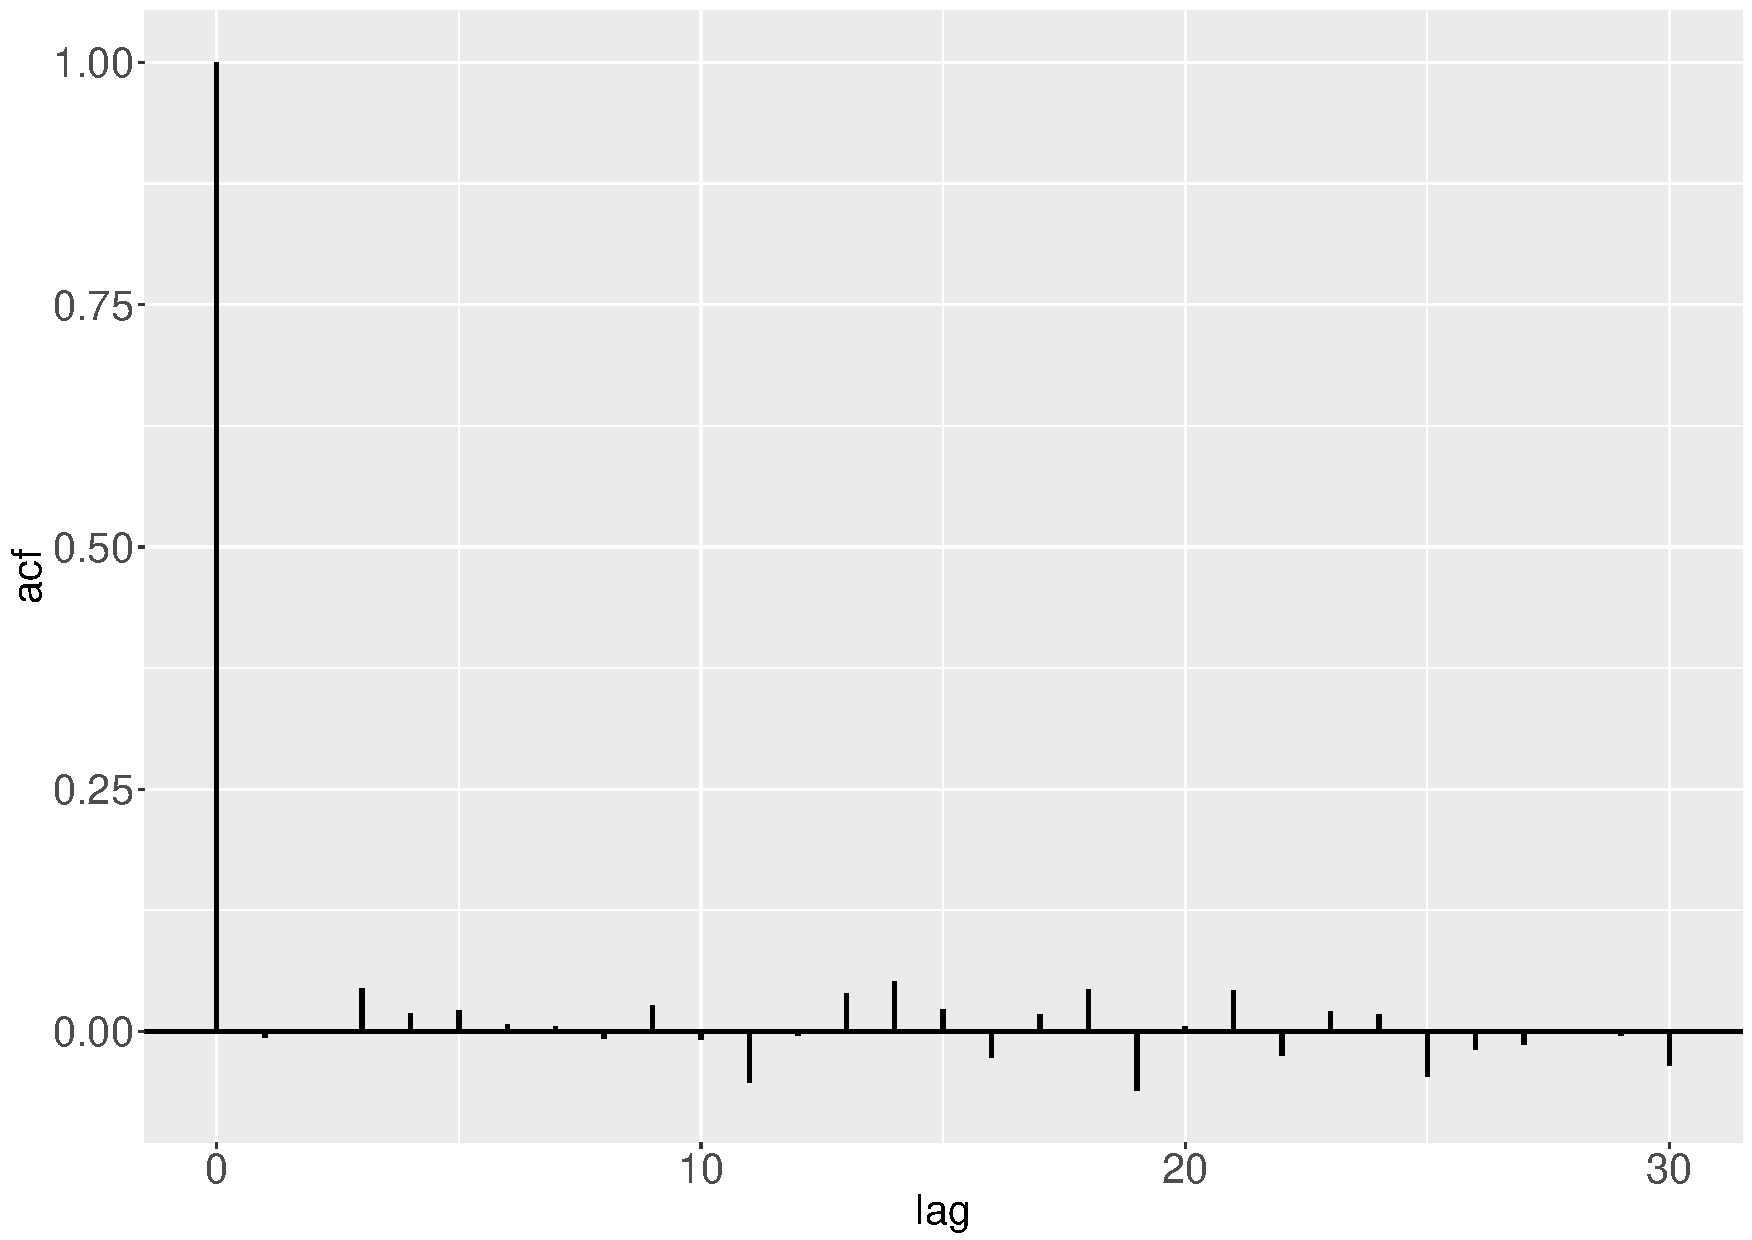
\includegraphics[width=\textwidth]{Chapters/02TractorSplineTheory/plot/ggplot/ggacfBlocks3.pdf}
    \caption{ACF of residuals from \textit{Blocks} with SNR at 3 }
    \end{subfigure}%
    \begin{subfigure}{0.45\textwidth}
    \centering
    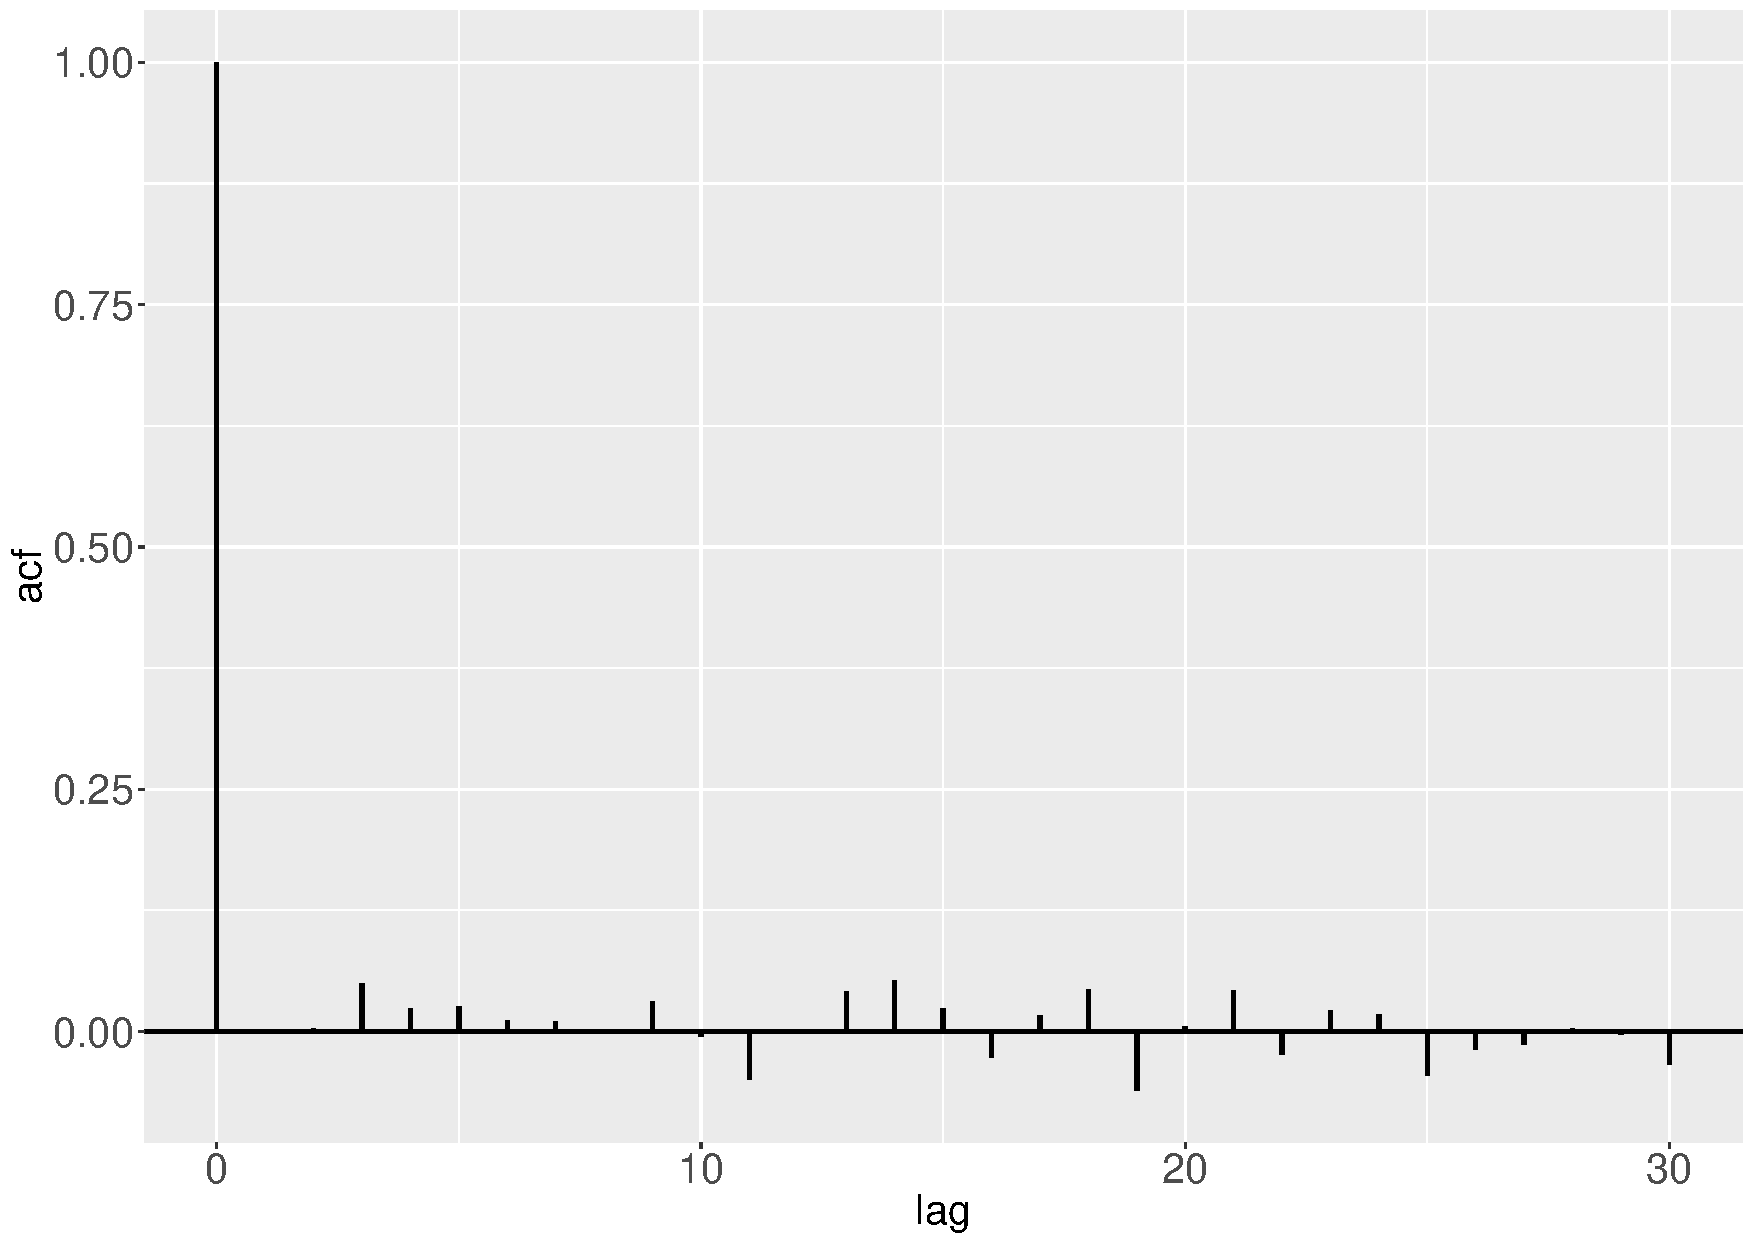
\includegraphics[width=\textwidth]{Chapters/02TractorSplineTheory/plot/ggplot/ggacfBumps3.pdf}
    \caption{ACF of residuals from \textit{Bumps} with SNR at 3 }
    \end{subfigure}
    \begin{subfigure}{0.45\textwidth}
    \centering
    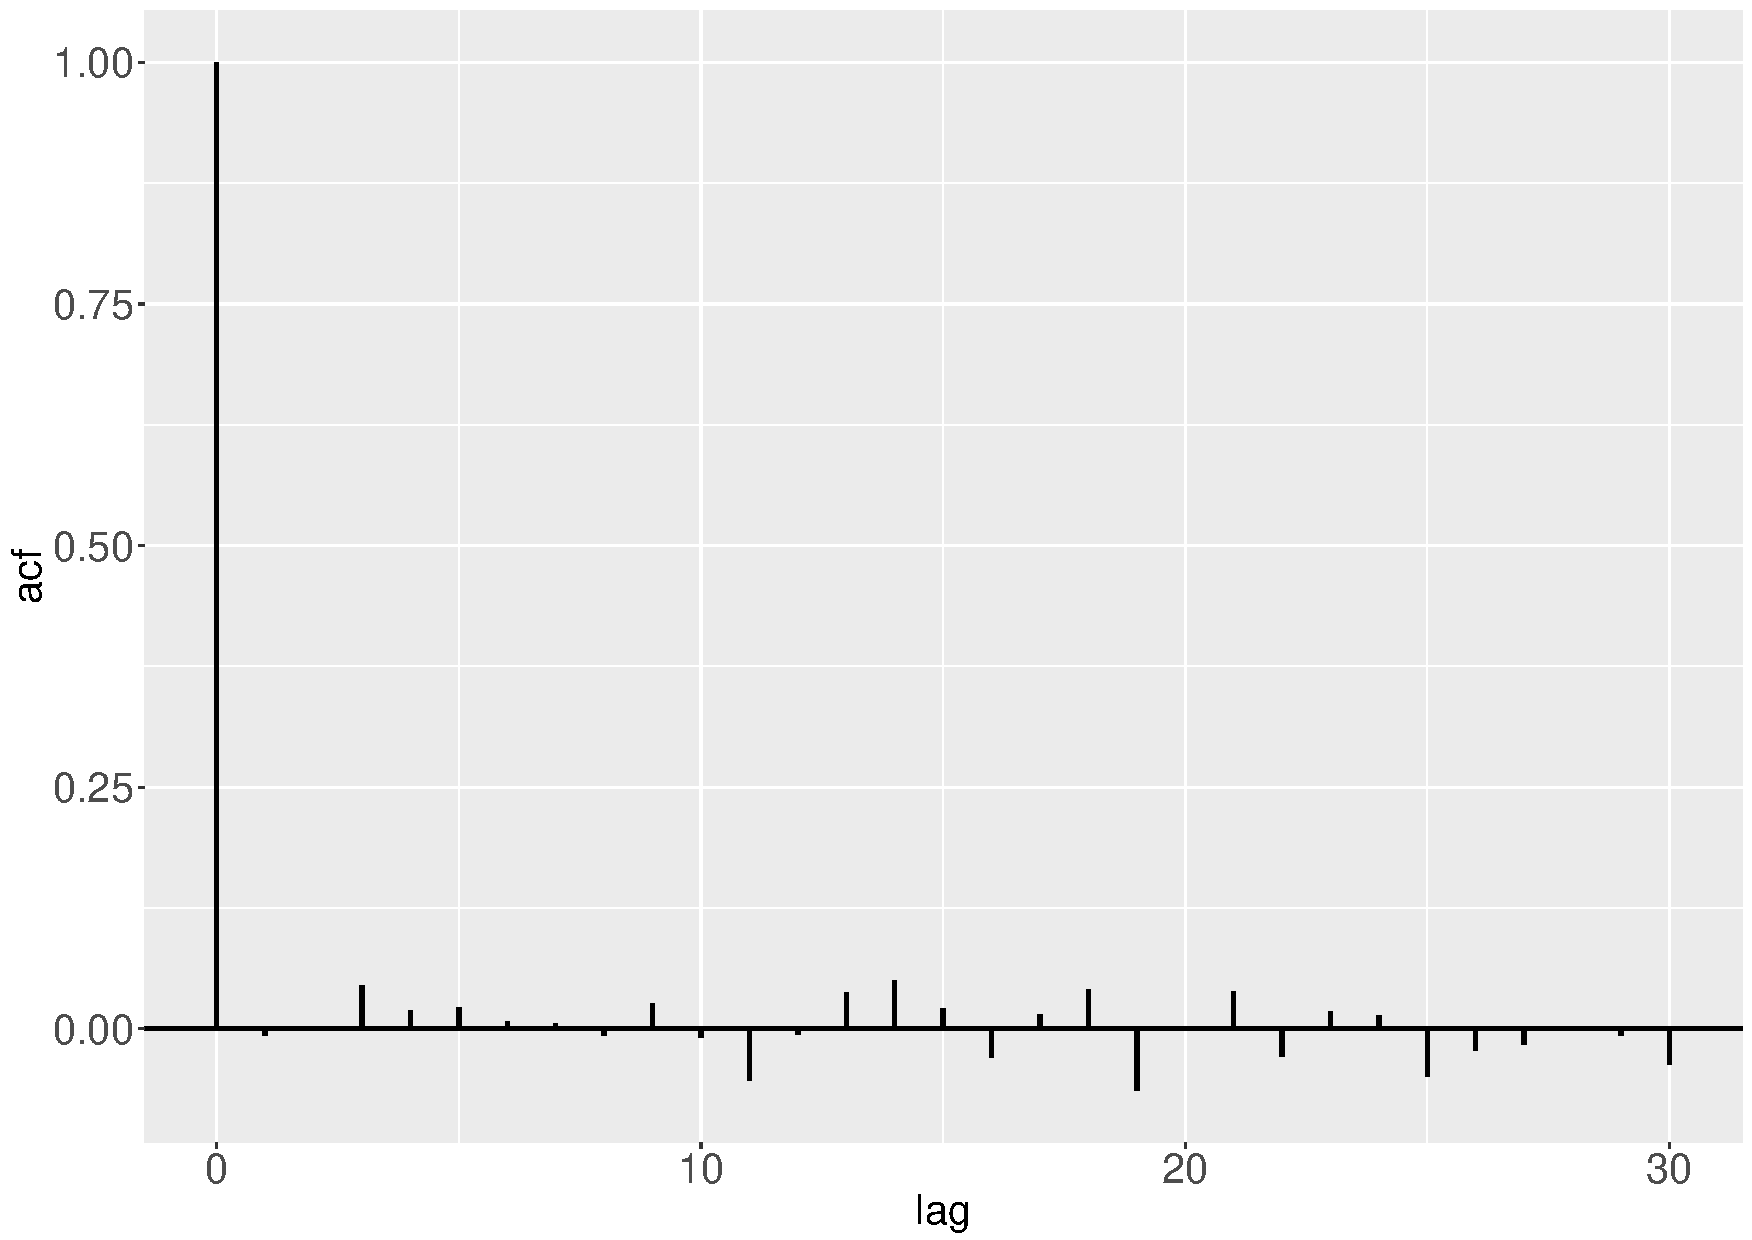
\includegraphics[width=\textwidth]{Chapters/02TractorSplineTheory/plot/ggplot/ggacfHeavi3.pdf}
    \caption{ACF of residuals from \textit{HeaviSine} with SNR at 3 }
    \end{subfigure}
    \begin{subfigure}{0.45\textwidth}
    \centering
    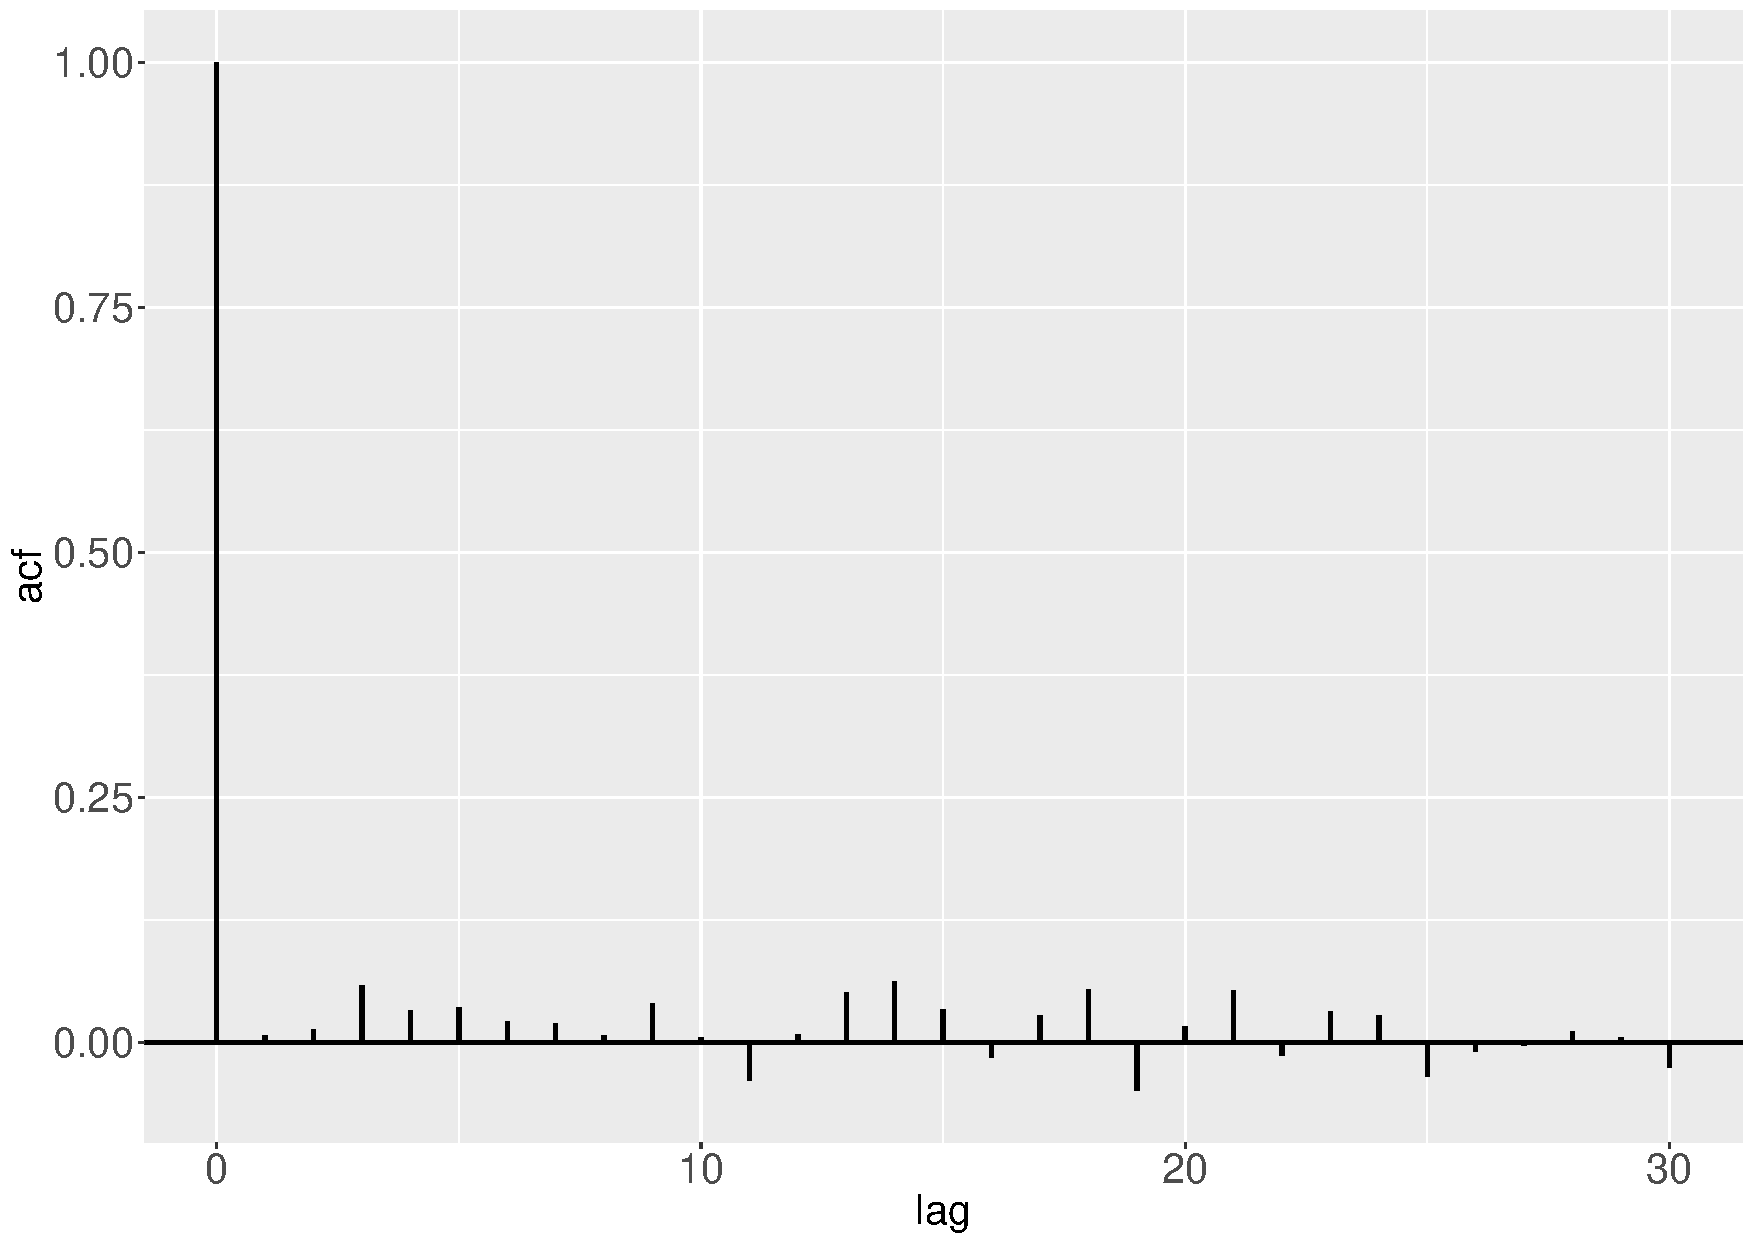
\includegraphics[width=\textwidth]{Chapters/02TractorSplineTheory/plot/ggplot/ggacfDoppler3.pdf}
    \caption{ACF of residuals from \textit{Doppler} with SNR at 3 }
    \end{subfigure}
\caption{ACF of residuals at SNR level of 3.}\label{tractorsplineSNR3acf}
 \end{figure}

\begin{figure}[!ht]
    \centering
    \begin{subfigure}{\textwidth}
    \centering
    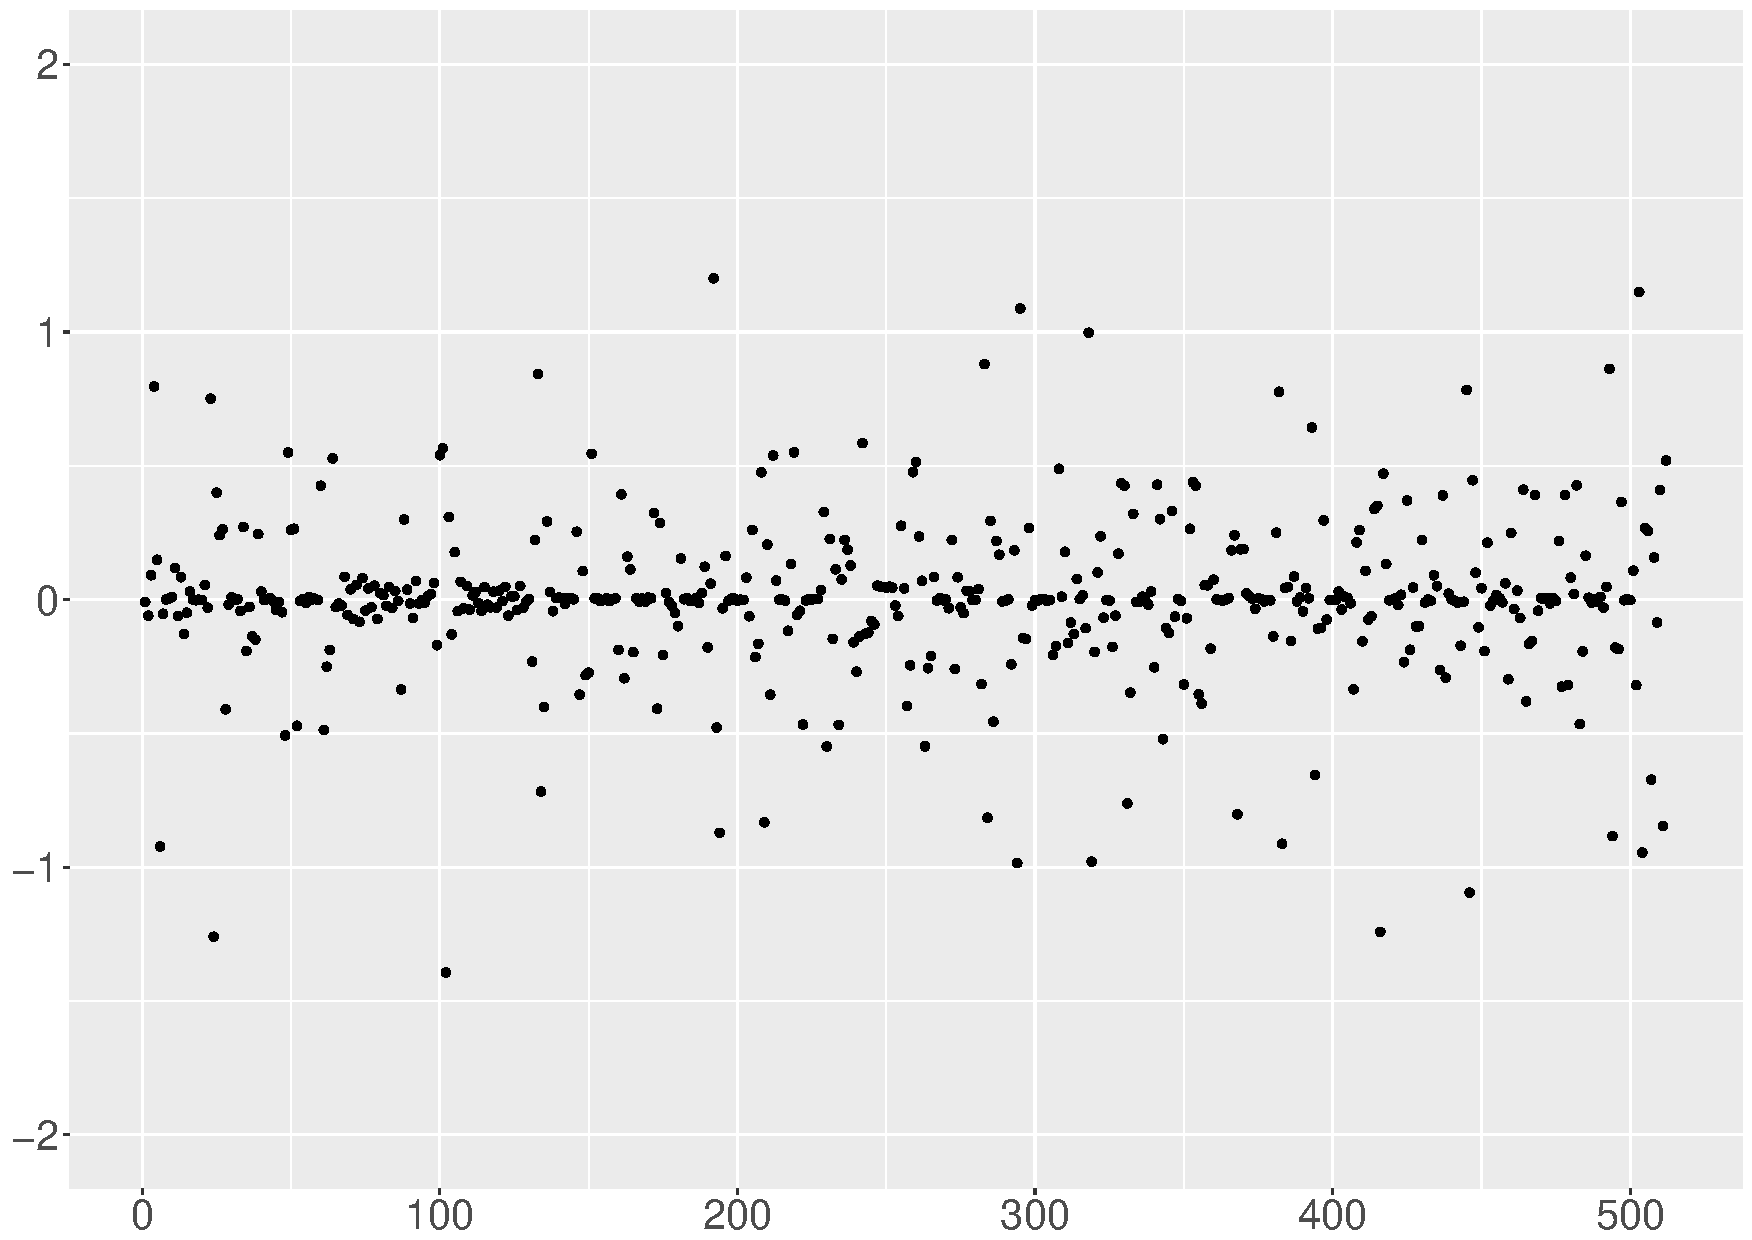
\includegraphics[width=0.45\linewidth]{Chapters/02TractorSplineTheory/plot/ggplot/ggRealdataXYResidualsXpoints.pdf}
    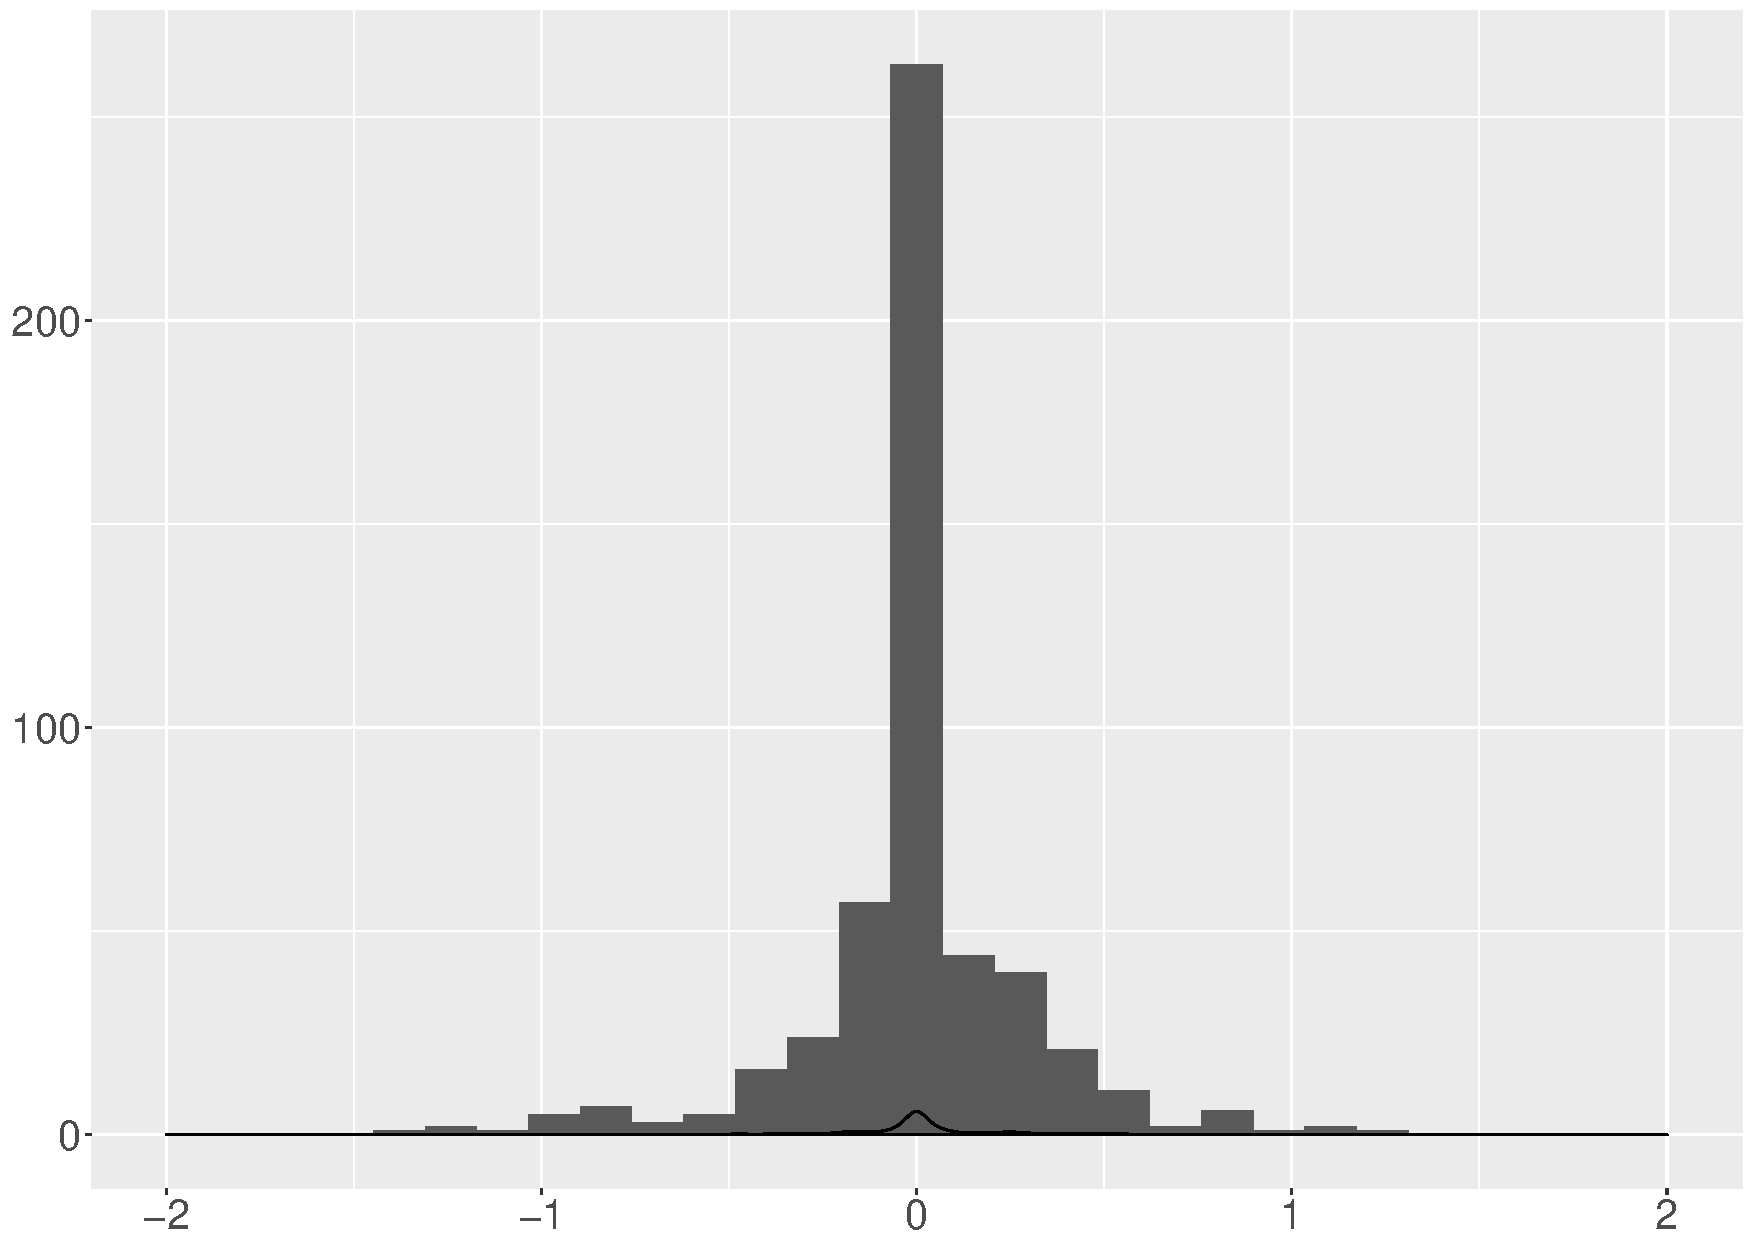
\includegraphics[width=0.45\linewidth]{Chapters/02TractorSplineTheory/plot/ggplot/ggRealdataXYResidualsXhist.pdf}
    \caption{residuals of $x$ }
    \end{subfigure}
    \begin{subfigure}{\textwidth}
    \centering
    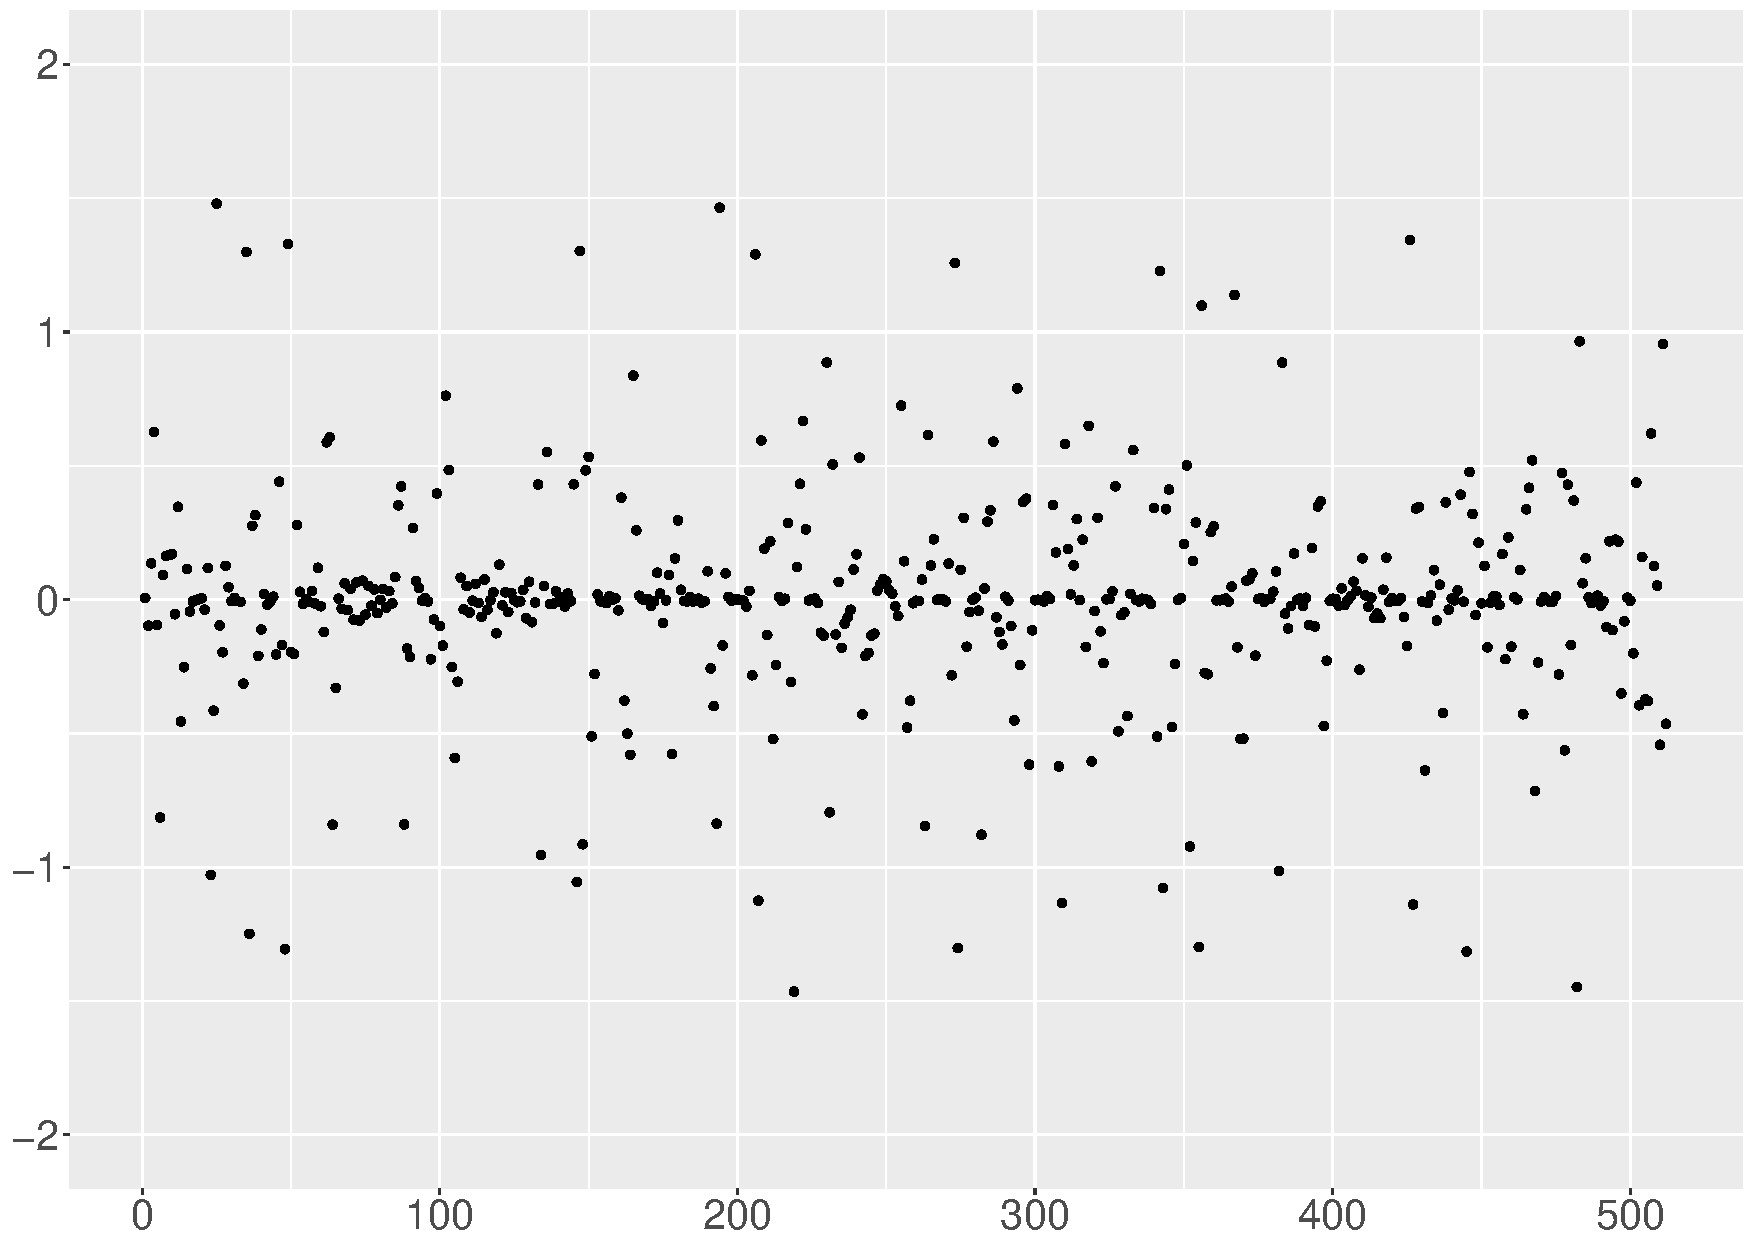
\includegraphics[width=0.45\linewidth]{Chapters/02TractorSplineTheory/plot/ggplot/ggRealdataXYResidualsYpoints.pdf}
    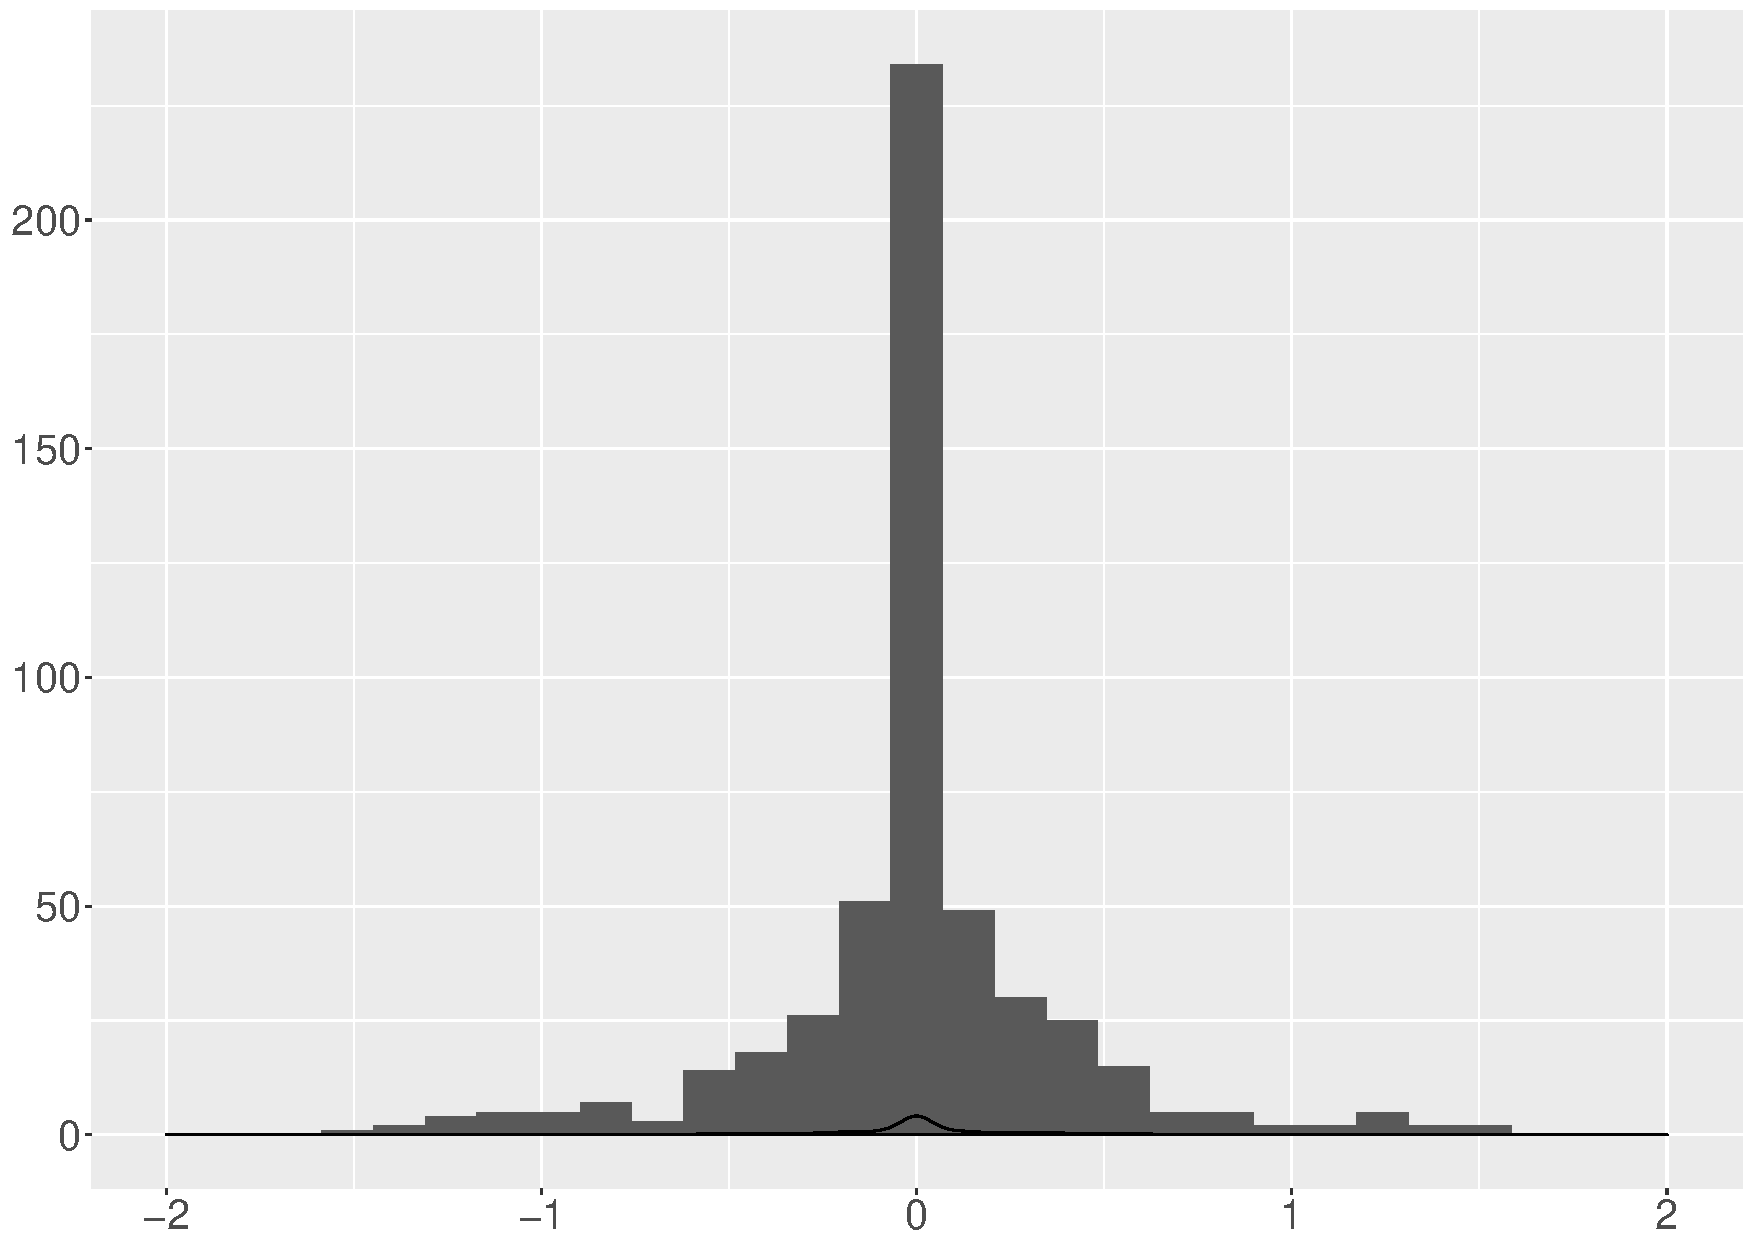
\includegraphics[width=0.45\linewidth]{Chapters/02TractorSplineTheory/plot/ggplot/ggRealdataXYResidualsYhist.pdf}
    \caption{residuals of $y$ }
    \end{subfigure}
\caption{Residuals of 2-dimensional real data reconstruction }\label{tractorsplineResidualsRealdata}
 \end{figure}

